% Template source: ICRA6_and_Risk_LatexTemplate.tex (ICRA template 2015, received from Montserrat Guillen)
% LaTeX documentation: https://www.latex-project.org/help/documentation/
% of which User's Guide: https://www.latex-project.org/help/documentation/usrguide.pdf
% Also check related links: https://www.latex-project.org/help/links/
% Comprehensive Tex Archive Network: https://www.ctan.org/

%***************************
% List of mathematical symbols: https://oeis.org/wiki/List_of_LaTeX_mathematical_symbols
%***************************

\documentclass[11pt,A4paper]{article}
%\documentclass[11pt,twoside,A4paper]{article}

\usepackage[papersize={21cm,29.7cm},left=3.5cm,top=3cm,right=3.5cm,bottom=2.5cm]{geometry}
\usepackage{latexsym,enumerate}
\usepackage{amsmath,amsthm,amsopn,amstext,amscd,amsfonts,amssymb}
\usepackage{graphics,graphicx}
\usepackage{setspace}
%\usepackage[spanish]{babel}
\usepackage[english]{babel}
\usepackage[T1]{fontenc}
\usepackage{uarial}
\renewcommand{\familydefault}{\sfdefault}
\usepackage{blindtext}
\usepackage{titlesec}

\usepackage{subfig}
\singlespace

\author{Daniel Mastropietro}
\title{Adaptive TD($\lambda$) in 1D gridworld}
\date{\today}

\begin{document}
\maketitle

\section{Introduction}

We consider a variation of the TD($\lambda$) algorithm where the choice of $\lambda$ is done in an adaptive way, based on the TD error observed at each time step, so that smaller TD errors give a value of $\lambda$ closer to 0 and larger TD errors give a value of $\lambda$ closer to 1.

A 1D gridworld with 21 states is considered as test bench, with its leftmost and rightmost states as terminal states giving respectively rewards equal to -1.0 and +1.0 when attained. All other state transitions give zero reward.

The agent follows the random walk policy and its goal is to estimate the state value function (prediction problem).

The algorithm is compared with two other learning algorithms:
\begin{itemize}
\item TD($\lambda$)
\item $\lambda$-return
\end{itemize}

\section{Adaptive TD($\lambda$) algorithm}

The algorithm proposes to adapt $\lambda$ at each learning time step by defining its value as a function of the TD error $\delta_t$:  

\medskip
$\delta_t = R_{t+1} + \gamma V(S_{t+1}) - V(S_t)$
\medskip

where $V(s)$ is the estimated state value function for state $s$, and $S_t$ is the state of the environment at time $t$, which is initially estimated equal to 0 for all states.

The value of $\lambda$ is now allowed to change at each time step $t$ and is proposed as a sigmoid function of the $\delta_t$ error *relative* to the estimated state value function at time $t$, namely:  

\medskip
$\lambda_t = 1 - exp(- |\delta^{rel}_t| )$  
\medskip

where $\delta^{rel}_t$ is given by:  

\begin{itemize}
\item $0$ if $V(S_t) = 0$ and $\delta_t = 0$  
\item $+\infty$ if $V(S_t) = 0$ and $\delta_t \neq 0$  
\item $\frac{\delta_t}{V(S_t)}$ o.w.  
\end{itemize}

Note that $\lambda_t \to 0^+$ when $\delta^{rel}_t \to 0$ and $\lambda_t \to 1^-$ when $|\delta^{rel}_t| \to +\infty$.

%This setup has the inconvenience that learning is slow at the beginning when the environment gives terminal-only rewards, as is the case here.

%For such scenarios, a burn-in like variant is used in some simulations, where 

%However, this adaptation is \emph{not} done for all time steps: in fact, in order to \emph{accelerate} the initial convergence of the algorithm for environments with terminal-only rewards (as is our case here), we begin by applying the traditional non-adaptive TD($\lambda$) algorithm

%the traditional non-adaptive TD($\lambda$) algorithm is applied at each time step as long as its next state has a \emph{value function that has %not been updated at least once}.

% This strategy has very much the spirit of a burn-in period that is run prior to starting the actual learning or estimation process. Similar results are expected to be obtained by not applying this strategy but instead setting the initial estimate of the state value function to sensibly selected random values.

\section{Learning rate}

In order to guarantee convergence of the algorithm, we apply a learning rate $\alpha(t)$ that satisfies the two convergence criteria of stochastic approximation algorithms, namely:

$\sum_{t} \alpha(t) = \infty$

$\sum_{t} \alpha^2(t) < \infty$

which are satisfied for instance with a law for $\alpha(t)$ that is proportional to $1/t$, for all $t \geq t_0$ for some positive $t_0$.

\section{Results}

For each of the three analyzed algorithms, we repeat 30 times the experiment of simulating the agent interaction with the gridworld environment using, at the onset of the simulation, the values of hyperparameters $\lambda$ and $\alpha$ that minimize the average root mean squared error (RMSE) over the first 10 episodes (obtained by running the simulation in one single experiment, which is the same for all three algorithms). For more details of this analysis see the `RL-001-MemoryManagement/SimulationTDLambda.ipynb` notebook.

In all cases, the initial estimate of the state value function is the constant zero function.

We then plot the RMSE at the end of each episode and compare their values among the three algorithms in order to analyse:  
\begin{itemize}
\item their early learning speed, for which we plot the RMSE at the end of each one out of the first 10 episodes
\item their convergence characteristics in the long run, for which we extend the above plot for the first 100 episodes.
\end{itemize}

The $\alpha$ parameter is set to its optimum at the beginning of the simulation, and is decreased as time proceeds. Letting $\alpha_0$ be the value of $\alpha$ at the onset of the simulation, we decrease its value proportional to the occupation number of each state, as long as the occupation number is at least 10, using the following expression:  

\medskip
$\alpha(S_t) = \frac{1}{(n(S_t) - 10) + 2}$  
\medskip

where $n(S_t)$ is the occupation number of state visited at time $t$ in each episode, $S_t$, \emph{since the start of the simulation process}. The adjustement of $\alpha$ is applied before the learning step at time $t$ takes place.

%\begin{enumerate}
%\item It is left unmodified for the first 10 episodes, and starting at the 11^{th} episode it is set equal to $\alpha_0/(k - 10 + 1)$, where $k$ %is the episode number starting at $1$.
%\item It is left unmodified for every state that has been visited less than 10 times during the simulation, and starting at the 10^{th} visit it %is set equal to $\alpha_0/(n(S_t) - 10 + 2)$, where $n(S_t)$ is the number of times the state visited at time $t$, $S_t$, has been visited so far.
%\item 
%\end{enumerate}

Figure \ref{fig:RMSE by episode} shows the evolution of the RMSE value obtained by the three analyzed learning algorithms applied to the 1D gridworld on the first 10 and first 100 episodes. The optimum hyperparameter values used in each case are displayed in the legend.

\begin{figure}[h!]
	\centering
	\subfloat[]{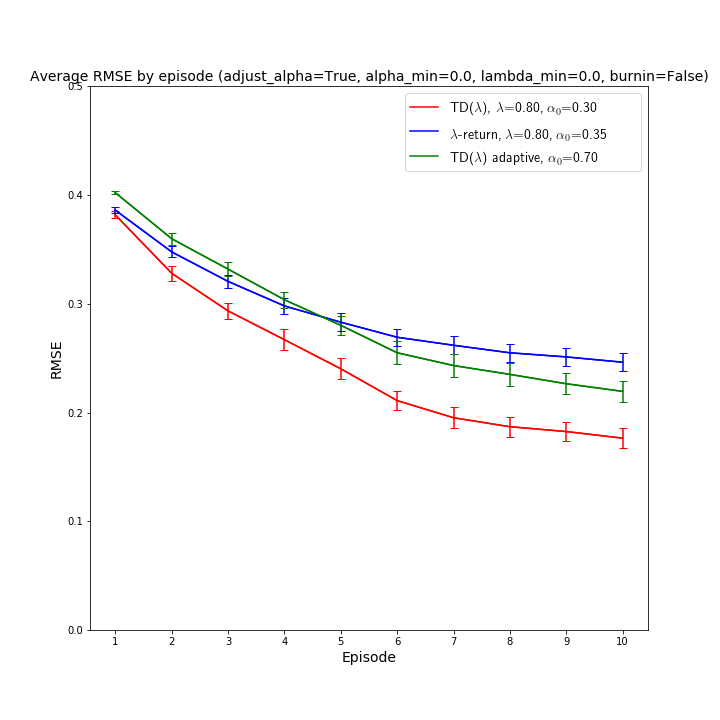
\includegraphics[width=0.5\linewidth]{results/SimulateTDLambda-Gridworld1D-AdaptiveTDLambda-v0.4-adjust_alpha=True,alpha_min=0.0,lambda_min=0.0,burnin=False-Episodes10.png}}
	\subfloat[]{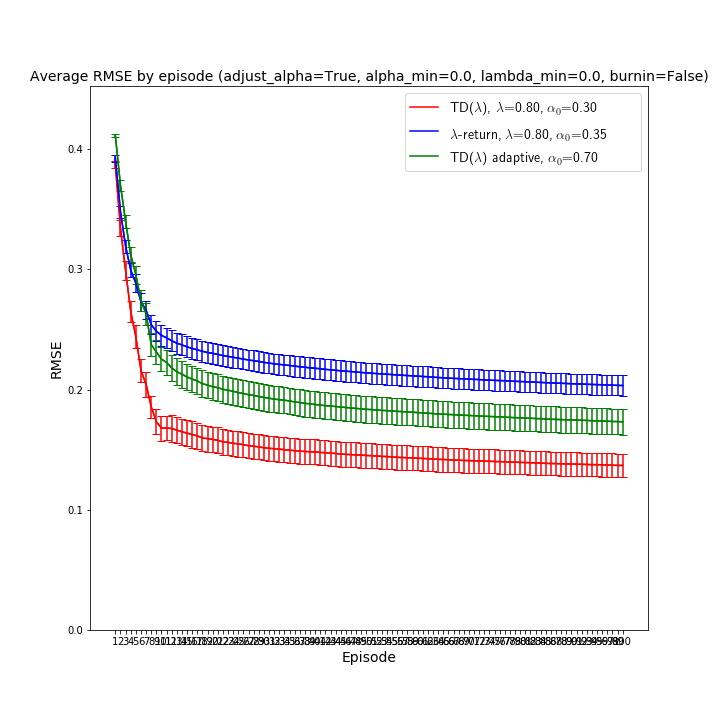
\includegraphics[width=0.5\linewidth]{results/SimulateTDLambda-Gridworld1D-AdaptiveTDLambda-v0.4-adjust_alpha=True,alpha_min=0.0,lambda_min=0.0,burnin=False-Episodes100.png}}
%		\caption{$\alpha$ is reduced as the inverse of the episode number exceeding 10, uniformly for all states.}
%		\caption{Learning speed: RMSE on the first 10 episodes.}
%	\begin{subfigure}{\linewidth}

%		\caption{$\alpha$ is reduced as the inverse of the state occupation starting at 10.}
%		\caption{Convergence analysis: RMSE on the first 100 episodes.}
%	\end{subfigure}
	\caption{RMSE by episode averaged over 30 experiments compared among the analyzed learning algorithms. The bars correspond to +/- one standard error. The green curve shows the performance of the adaptive TD($\lambda$) algorithm.  (a) Learning speed: RMSE on the first 10 episodes. (b) Convergence analysis: RMSE on the first 100 episodes.}
	\label{fig:RMSE by episode}
\end{figure}


We observe a slower convergence of the adaptive TD($\lambda$) than the other two algorithms at the start of the simulation, and a larger error in the long-run than the traditional TD($\lambda$). This is not surprising considering that this is a terminal-only reward environment and, at the onset, the state value function estimate is set to 0 for all states. Under this scenario, $\lambda_t$ becomes 0 for most of the states far away from the terminal states, as the TD error is 0, until the non-zero reward information reaches one of their neighbouring states. In addition, in the long run, once the value function estimates become more stable as time passes, there is less innovation observed at each episode run, and therefore $\lambda$ becomes again close to 0.

To remedy this problem, we shrink the range of variation of $\lambda_t$ to  $[0.1, 1)$ (by multiplying the exponential in the original formula by $(1 - 0.1)$), so that a small \emph{but non-zero} $\lambda$ is guaranteed when the innovation information in the TD error is small. The results under this setup are shown in Figure \ref{fig:RMSE by episode with min lambda}.

%\begin{figure}[h!]
%	\centering
%	\subfloat[]{\includegraphics[width=0.5\linewidth]{results/SimulateTDLambda-Gridworld1D-AdaptiveTDLambda-v0.4-%adjust_alpha=True,alpha_min=0.0,lambda_min=0.0,burnin=True-Episodes10.png}}
%	\subfloat[]{\includegraphics[width=0.5\linewidth]{results/SimulateTDLambda-Gridworld1D-AdaptiveTDLambda-v0.4-%adjust_alpha=True,alpha_min=0.0,lambda_min=0.0,burnin=True-Episodes100.png}}
%	\caption{RMSE by episode compared among the analyzed learning algorithms. Modified adaptive TD($\lambda$) algorithm: with burn-in. (a) %Learning speed: RMSE on the first 10 episodes. (b) Convergence analysis: RMSE on the first 100 episodes.}
%	\label{fig:RMSE by episode}
%\end{figure}


\begin{figure}[h!]
	\centering
	\subfloat[]{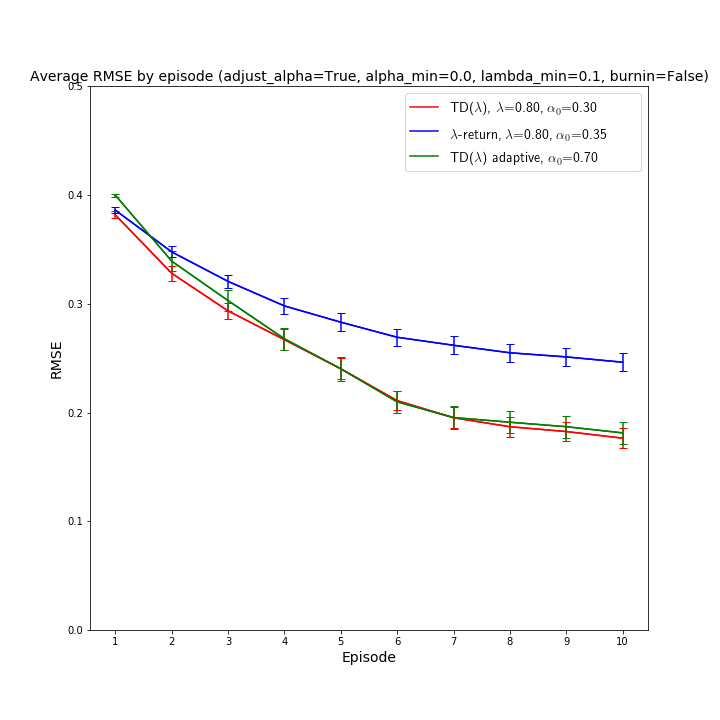
\includegraphics[width=0.5\linewidth]{results/SimulateTDLambda-Gridworld1D-AdaptiveTDLambda-v0.4-adjust_alpha=True,alpha_min=0.0,lambda_min=0.1,burnin=False-Episodes10.png}}
	\subfloat[]{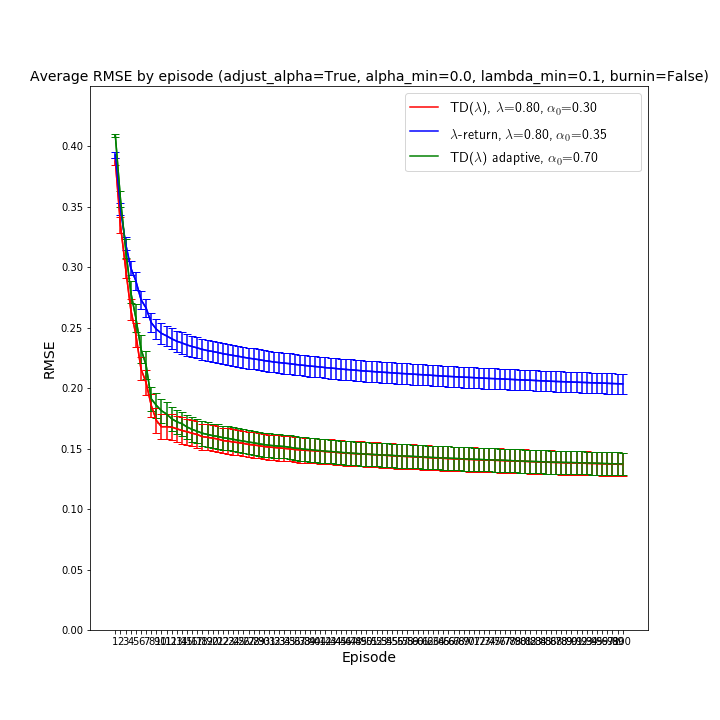
\includegraphics[width=0.5\linewidth]{results/SimulateTDLambda-Gridworld1D-AdaptiveTDLambda-v0.4-adjust_alpha=True,alpha_min=0.0,lambda_min=0.1,burnin=False-Episodes100.png}}
	\caption{RMSE by episode averaged over 30 experiments compared among the analyzed learning algorithms. The bars correspond to +/- one standard error. The green curve shows the performance of the adaptive TD($\lambda$) algorithm, modified to a $\lambda_t$'s range in the interval $[0.1, 1)$. (a) Learning speed: RMSE on the first 10 episodes. (b) Convergence analysis: RMSE on the first 100 episodes.}
	\label{fig:RMSE by episode with min lambda}
\end{figure}


%\begin{figure}[h!]
%	\centering
%	\subfloat[]{\includegraphics[width=0.4\linewidth]{results/SimulateTDLambda-Gridworld1D-AdaptiveTDLambda-v0.4-%adjust_alpha=True,alpha_min=0.1,lambda_min=0.0,burnin=False-Episodes10.png}}
%	\subfloat[]{\includegraphics[width=0.4\linewidth]{results/SimulateTDLambda-Gridworld1D-AdaptiveTDLambda-v0.4-%adjust_alpha=True,alpha_min=0.1,lambda_min=0.0,burnin=False-Episodes100.png}}
%	\caption{RMSE by episode compared among the analyzed learning algorithms. Modified adaptive TD($\lambda$) algorithm: $\alpha(S_t) \geq 0.10$. %(a) Learning speed: RMSE on the first 10 episodes. (b) Convergence analysis: RMSE on the first 100 episodes.}
%	\label{fig:RMSE by episode}
%\end{figure}


In this case the performance is very similar to the traditional TD($\lambda$) both in the short run and in the long run, with the advantage that there is one less hyperparameter to determine, namely $\lambda$. Although we still need to set a value for the minimum accepted $\lambda$ (0.1 in this case), it is expected that the algorithm performance is not too sensitive to this value.


\newpage

\bibliography{RL}
\bibliographystyle{plain}




\iffalse

\medskip
It is assumed that:

\[S \sim \epsilon(\lambda)\]
\[T \sim \epsilon(1/\tau)\]

\subsection{Detection with noise}
The experiment is prone to several sources of errors. One of them is the following: from time to time the arrival of a new muon may be \textit{incorrectly classified} as a decay detection, thus causing an incorrect measurement of the muon's decay time.

\medskip
In order to model different sources of error, let us define the following random variable:

$U$: "Decay time of a muon in the presence of \textit{noise}"

where the \textit{noise} is generated by the incorrect detection of a muon decay.

\medskip
How is $U$ distributed?

\[ \\
U =
\left \{
  \begin{tabular}{ll}
  $T$ & \textrm{if it's a genuine decay detection} \\
  $S$ & \textrm{if the decay time measurement was triggered by the arrival of another muon} \\
  \end{tabular}
\right.
\]

\begin{align*}
F_U(u) 	= P(U \leq u) 	= & P(T \leq u /Y\!=\!0) \; (1-p) + P(S \leq u /Y\!=\!1) \; p \\
						= & (1 - e^{-u/\tau}) \; 1/(1 + \lambda \tau) I\{u \geq 0\} + 
							(1 - e^{-\lambda u}) \; \lambda \tau /(1 + \lambda \tau) I\{u \geq 0\} \\
						\approx & (1 - e^{-u/\tau}) \; (1 - \lambda \tau) I\{u \geq 0\} +
							 (1 - e^{-\lambda u}) \; \lambda \tau I\{u \geq 0\}
\end{align*}

\[
f_U(u) = F'_U(u) \approx \left[ \frac{(1 - \lambda \tau)}{\tau} e^{-u/\tau} \; + \lambda^2 \tau e^{-\lambda u} \; \right] I\{u \geq 0\}
\textrm{ when } \lambda \tau << 1.
\]

Note that as $\lambda \tau \to 0, f_U(u) \to \frac{e^{-u/\tau}}{\tau} \; I\{u \geq 0\} = f_T(u)$, that is $U$ tends to be distributed as $T$.

\subsection{Maximum Likelihood estimation of the parameters}
\[
l(\lambda, \tau / \underline{u}) = \sum_{i=1}^{n} \log \left[ \frac{(1 - \lambda \tau)}{\tau} e^{-u_i/\tau} \; + \lambda^2 \tau e^{-\lambda u_i} \; \right]
\]

or equivalently:

\[
l(\lambda, \tau / \underline{u}) = -\lambda \sum_{i=1}^{n} u_i + 
											\sum_{i=1}^{n} {\log \left[ \frac{(1 - \lambda \tau)}{\tau} e^{-\frac{(1 - \lambda \tau)}{\tau} u_i} \; + \lambda^2 \tau \; \right]}
\]

\fi

\end{document}
